\documentclass[a4paper,12pt,twoside]{memoir}

% Castellano
\usepackage[spanish,es-tabla]{babel}
\selectlanguage{spanish}
\usepackage[utf8]{inputenc}
\usepackage[T1]{fontenc}
\usepackage{lmodern} % scalable font
\usepackage{microtype}
\usepackage{placeins}

\RequirePackage{booktabs}
\RequirePackage[table]{xcolor}
\RequirePackage{xtab}
\RequirePackage{multirow}

% Links
\PassOptionsToPackage{hyphens}{url}\usepackage[colorlinks]{hyperref}
\hypersetup{
	allcolors = {red}
}
\usepackage{url}

% Ecuaciones
\usepackage{amsmath}

% Rutas de fichero / paquete
\newcommand{\ruta}[1]{{\sffamily #1}}

% Párrafos
\nonzeroparskip

% Huérfanas y viudas
\widowpenalty100000
\clubpenalty100000

% Evitar solapes en el header
\nouppercaseheads


\let\tmp\oddsidemargin
\let\oddsidemargin\evensidemargin
\let\evensidemargin\tmp
\reversemarginpar



% Imagenes
\usepackage{graphicx}
\newcommand{\imagen}[2]{
	\begin{figure}[!h]
		\centering
		\includegraphics[width=0.9\textwidth]{#1}
		\caption{#2}\label{fig:#1}
	\end{figure}
	\FloatBarrier
}






\graphicspath{ {./img/} }

% Capítulos
\chapterstyle{bianchi}
\newcommand{\capitulo}[2]{
	\setcounter{chapter}{#1}
	\setcounter{section}{0}
	\setcounter{figure}{0}
	\setcounter{table}{0}
	\chapter*{#2}
	\addcontentsline{toc}{chapter}{#2}
	\markboth{#2}{#2}
}

% Apéndices
\renewcommand{\appendixname}{Apéndice}
\renewcommand*\cftappendixname{\appendixname}

\newcommand{\apendice}[1]{
	%\renewcommand{\thechapter}{A}
	\chapter{#1}
}

\renewcommand*\cftappendixname{\appendixname\ }

% Formato de portada
\makeatletter
\usepackage{xcolor}
\newcommand{\tutor}[1]{\def\@tutor{#1}}
\newcommand{\tutorb}[1]{\def\@tutorb{#1}}
\newcommand{\course}[1]{\def\@course{#1}}
\definecolor{cpardoBox}{HTML}{E6E6FF}
\def\maketitle{
  \null
  \thispagestyle{empty}
  % Cabecera ----------------
\begin{center}
  \noindent\includegraphics[width=\textwidth]{cabeceraSalud}\vspace{1.5cm}%
\end{center}
  
  % Título proyecto y escudo salud ----------------
  \begin{center}
    \begin{minipage}[c][1.5cm][c]{.20\textwidth}
        \includegraphics[width=\textwidth]{escudoSalud.pdf}
    \end{minipage}
  \end{center}
  
  \begin{center}
    \colorbox{cpardoBox}{%
        \begin{minipage}{.8\textwidth}
          \vspace{.5cm}\Large
          \begin{center}
          \textbf{TFG del Grado en Ingeniería de la Salud}\vspace{.6cm}\\
          \textbf{\LARGE\@title{}}
          \end{center}
          \vspace{.2cm}
        \end{minipage}
    }%
  \end{center}
  
    % Datos de alumno, curso y tutores ------------------
  \begin{center}%
  {%
    \noindent\LARGE
    Presentado por \@author{}\\ 
    en Universidad de Burgos\\
    \vspace{0.5cm}
    \noindent\Large
    \@date{}\\
    \vspace{0.5cm}
    %Tutor: \@tutor{}\\ % comenta el que no corresponda
    Tutores: \@tutor{} -- \@tutorb{}\\
  }%
  \end{center}%
  \null
  \cleardoublepage
  }
\makeatother



% Datos de portada
\title{ASMR Sleep. Aplicación de recomendación y análisis de vídeos destinada a pacientes con Insomnio de Conciliación. \\Documentación Técnica}
\author{Rocío Alonso las Heras}
\tutor{Antonio Jasús Canepa Oneto}
\tutorb{Estefanía Rivas Navas}
\date{\today}

\begin{document}

\maketitle



\cleardoublepage



%%%%%%%%%%%%%%%%%%%%%%%%%%%%%%%%%%%%%%%%%%%%%%%%%%%%%%%%%%%%%%%%%%%%%%%%%%%%%%%%%%%%%%%%



\frontmatter


\clearpage

% Indices
\tableofcontents

\clearpage

\listoffigures

\clearpage

\listoftables

\clearpage

\mainmatter

\appendix
\apendice{Apéndice A. Planificación Temporal del Proyecto}
\section{Introducción}
El presente Trabajo de Fin de Grado fue inicialmente propuesto en septiembre, comenzando formalmente su desarrollo en diciembre. El proyecto tiene una duración total de 25 semanas, correspondiente a 15 ECTS. De acuerdo con la normativa académica, cada crédito ECTS representa aproximadamente 25 a 30 horas de trabajo, lo que se traduce en un total de entre 375 y 450 horas, tomadas de manera orientativa, dedicadas al trabajo.

Para gestionar eficazmente el tiempo y las tareas, se ha utilizado el método Scrum, descrito en la memoria. Esta planificación temporal ha servido de guía para distribuir las horas de trabajo a lo largo de las 25 semanas, asegurando una adecuada progresión y finalización del proyecto dentro del plazo establecido.

La planificación temporal se ha estructurado en sprints de una semana, cada uno con objetivos específicos, permitiendo una evaluación continua del avance y ajustes necesarios para cumplir con los requisitos del TFG. A continuación, se presenta un calendario general por semanas y se detalla la planificación de cada sprint.

\begin{figure}
    \centering
    \includegraphics[width=1\textwidth]{imagenes/calendariobien.png}
    \caption{Calendario Planificación temporal}
    \label{fig:enter-label}
\end{figure}

\section{Planificación Temporal}
En esta sección se detallará la planificación original de los sprints por semanas, comenzando el 11 de diciembre y finalizando el 20 de junio, de manera gráfica mediante una tabla, y con una descripción de las tareas por sprint.

\begin{itemize}
    \item \textbf{Semana 1}
    \begin{enumerate}
        \item Planificación del proyecto
        \item Formalización de la idea
        \item Creación del calendario
    \end{enumerate}
    \item \textbf{Semana 2}
    \begin{enumerate}
        \item Autenticación en Youtube
        \item Creación del proyecto en Google Console
        \item Definición de la aplicación en Google Console
    \end{enumerate}
    \item \textbf{Semana 3}
    \begin{enumerate}
        \item Habilitación Youtube Data API
        \item Obtención de credenciales para la autenticación
    \end{enumerate}
    \item \textbf{Semana 4}
    \begin{enumerate}
        \item Comprensión paquete \textbf{\textit{tuber}} en R
    \end{enumerate}
    \item \textbf{Semana 5}
    \begin{enumerate}
        \item Prueba de la función \textit{yt auth}
    \end{enumerate}
    \item \textbf{Semana 6}
    \begin{enumerate}
        \item Establecimiento de conexión entre YouTube Data API y R
    \end{enumerate}
    
    \item \textbf{Semana 7}
    \begin{enumerate}
        \item Pruebas de primeras búsquedas desde R
        \item Resolución de errores en las consultas
    \end{enumerate}
    \item \textbf{Semana 8}
    \begin{enumerate}
        \item Gestión salida de datos de las consultas
        \item Selección de criterios de búsqueda relevantes
        \item Documentación errores en la autenticación
    \end{enumerate}
    \item \textbf{Semana 9}
    \begin{enumerate}
        \item Gestión salida de datos de las consultas
        \item Selección de criterios de búsqueda relevantes
        \item Documentación errores en la autenticación
    \end{enumerate}
    \item \textbf{Semana 10}
    \begin{enumerate}
        \item Comparación de datos y estadisticas obtenibles en función del método
        \item Selección del método óptimo de búsqueda y guardado de datos
        \item Definición de objetivos de la aplicación
    \end{enumerate}
    \item \textbf{Semana 11}
    \begin{enumerate}
        \item Definición ASMR
        \item Explicación del fenómeno y su historia
        \item Descripción básica de los principales estímulos o \textit{Triggers}
        \item Bocetado inicial de la UI (Interfaz de Usuario)
        \item Bocetado de esquemas de estructura y flujo de la aplicación
        \end{enumerate}
    \item \textbf{Semana 12}
    \begin{enumerate}
        \item Búsqueda de literatura sobre el sueño
        \item Búsqueda de literatura sobre el insomnio
        \item Búsqueda de literatura sobre terapias convencionales y alternativas
        \item Creación de esquemas de los casos de uso de la aplicación
        \end{enumerate}
    \item \textbf{Semana 13}
    \begin{enumerate}
        \item Análisis teórico insomnio de conciliación
        \item Estudio sobre tipos de insomnio
        \item Caracterización del diagnóstico diferencial del insomnio de conciliación
        \item Descripción de los casos de uso de la aplicación
    \end{enumerate}
    \item \textbf{Semana 14}
    \begin{enumerate}
        \item Teoría tratamiento del Insomnio
        \item Diferenciación tratamientos farmacológicos y no farmacológicos
        \item Indagación terapias alternativas
        \item Definición de las bases de datos
    \end{enumerate}
    \item \textbf{Semana 15}
    \begin{enumerate}
        \item Teoría tratamiento del Insomnio
        \item Diferenciación tratamientos farmacológicos y no farmacológicos
        \item Indagación terapias alternativas
        \item Esquemas de las bases de datos
    \end{enumerate}
    \item \textbf{Semana 16}
    \begin{enumerate}
        \item Teoría tratamiento del Insomnio
        \item Diferenciación tratamientos farmacológicos y no farmacológicos
        \item Indagación terapias alternativas
        \item Implementación de la búsqueda
    \end{enumerate}
    \item \textbf{Semana 17}
    \begin{enumerate}
        \item Creación pestaña de inicio para usuarios
        \item Prueba de escritura de nuevos usuarios sobre la base de datos
    \end{enumerate}
    \item \textbf{Semana 18}
    \begin{enumerate}
        \item Creación de pestaña de administrador
        \item Implementación operaciones \textit{CRUD}
    \end{enumerate}
    \item \textbf{Semana 19}
    \begin{enumerate}
        \item Selección \textit{triggers} para la pestaña de preferencias
        \item Creación de pestaña de preferencias
    \end{enumerate}
    \item \textbf{Semana 20}
    \begin{enumerate}
        \item Selección de criterios para la pestaña de estadísticas
        \item Creación de pestaña de estadísticas
    \end{enumerate}
    \item \textbf{Semana 21}
    \begin{enumerate}
        \item Unión de pestañas 
        \item Correccion de errores
    \end{enumerate}
    \item \textbf{Semana 22}
    \begin{enumerate}
        \item Realizacion de pruebas de funcionalidad
        \item Realización de pruebas de rendimiento
    \end{enumerate}
    \item \textbf{Semana 23}
    \begin{enumerate}
        \item Identificación de mejoras y errores
    \end{enumerate}
    \item \textbf{Semana 24}
    \begin{enumerate}
        \item Redacción formal del informe
    \end{enumerate}
    \item \textbf{Semana 25}
    \begin{enumerate}
        \item Redacción formal de Anexos
    \end{enumerate}
    \item \textbf{Semana 26}
    \begin{enumerate}
        \item Margen de mejoras
    \end{enumerate}
    \item \textbf{Semana 27}
    \begin{enumerate}
        \item Entrega del proyecto
    \end{enumerate}
    \item \textbf{Semana 28}
    \begin{enumerate}
        \item Defensa del proyecto
    \end{enumerate}
\end{itemize}

Esta planificación es una muestra mixta entre la planificación inicial y la que resultó llevarse a cabo, dado que algunas cosas cambiaron de posición en base a su importancia en el desarrollo, y a que en los sprints se mantienen las tareas no resueltas de un sprint para el siguiente.

\section{Viabilidad Económica}
Esta sección describe los costes y beneficios relativos a este proyecto, descritos de manera hipotética. Los aspectos a tener en cuenta son
\begin{itemize}
    \item Localización: El proyecto fue desarrollado en Burgos, pero los costes son extrapolables a toda España.
    \item Duración del proyecto: La duración real del proyecto fueron 6 meses.
    \item Equipo de desarrollo: La desarrolladora principal del proyecto fue la alumna, se calcularán los costes simulando que se tratase de un proyecto autónomo.
\end{itemize}
\subsection{Costes de personal}
Los costes de personal son aquellos derivados del salario de los participantes en el proyecto, en este caso solamente 1, conformados por el salario bruto, la retención por IRPF y la Seguridad Social.

El salario ha sido basado en la premisa de la alumna trabajando como programadora junior, con el salario medio en España de este rol. Y dando un tiempo de 5 meses de realización, no teniendo en cuenta el tiempo de documentación académica del proyecto. \cite{salariopj}

\begin{table}[h!]
\centering
\begin{tabular}{llll}
\toprule
Concepto & Coste & Tiempo & Cantidad \\
\midrule
Salario neto & 1.750 & 5 meses & 8.750 €\\
IRPF & 18\% & 5 meses & 1.575 €\\
Seguridad social & 29.9\% & 5 meses & 3.558,1 €\\
Total costes personal & & & 13.883,1 €\\
\end{tabular}
\caption{Costes personal}
\label{tabla-costes personal}
\end{table}


\subsection{Costes de hardware}
El único hardware utilizado ha sido el ordenador portátil desde el que el proyecto ha sido desarrollado, se toma como modelo el utilizado, \textit{Asus Vivobook 15}, calculando un valor amortizado a 5 años, teniendo en cuenta que el proyecto ha durado 6 meses.

\begin{table}[h!]
\centering
\begin{tabular}{lll}
\toprule
Material & Coste & Amortizado\\
\midrule
Ordenador portátil & 849 € & 84,9 €\\
\end{tabular}
\caption{Costes hardware}
\label{tabla-hardware}
\end{table}

\subsection{Costes de software}

No se tienen en cuenta costes de software dado que todos los programas utilizados han sido de licencia abierta o bajo licencia educativa. En caso de que el proyecto se monetizase podrían mejorarse algunas de las opciones, accediendo a la versión de pago de Google Console o externalizando las bases de datos, lo que aumentaría los costes.

\subsection{Costes generales}
En cuanto a los costes generales del proyecto, estos son los derivados del uso de una oficina.

\begin{table}[h!]
\centering
\begin{tabular}{llll}
\toprule
Concepto & Coste & Tiempo & Cantidad \\
\midrule
Alquiler & 400 € & 5 meses & 2.000 €\\
Luz & 50 € & 5 meses & 250 €\\
Agua & 20 € & 5 meses & 100 €\\
Internet & 40 € & 5 meses & 200 €\\
Total costes generales & & & 2.550 €\\
\end{tabular}
\caption{Costes generales}
\label{tabla-costes generales}
\end{table}

\subsection{Costes totales}
Los costes derivados de la suma de los anteriores.
\begin{table}[h!]
\centering
\begin{tabular}{ll}
\toprule
Coste & Total\\
\midrule
Personal & 13.883,1 €\\
Hardware & 84,9 €\\
Oficina & 2.550 €\\
Software & 0 €\\
\textbf{Total} & 16.518 €\\
\end{tabular}
\caption{Costes Totales}
\label{tabla-costes}
\end{table}
\subsection{Beneficios}
Esta aplicación fue concebida como una medida gratuita y accesible para los pacientes, sin anuncios, por lo que la idea inicial no reporta beneficios, si no derivan de una ayuda como medida sanitaria. \\
De manera hipotética se podría plantear la idea de que los creadores de contenido ASMR pagasen por que sus vídeos apareciesen en la aplicación, lo que permitiría costearla.

\section{Viabilidad legal}
La viabilidad legal del proyecto, regulado bajo el marco de la legislación española, ha de atender a las siguientes leyes:
\begin{itemize}
    \item Real Decreto Legislativo 1/1996 \cite{boe1996} relativo Ley de Propiedad Intelectual y Ley 24/2015, Ley de Patentes, en cuanto a los derechos de autoría del proyecto. \cite{Ley24/2015}
    \item Ley Orgánica 3/2018, de 5 de diciembre, de Protección de Datos Personales y Garantía de los Derechos Digitales. \cite{boe-2018} En cuanto al tratamiento de los datos de los usuarios.
    \item Leyes reguladoras de los trabajadores como Ley de Protección de Riesgos Laborales y Estatuto de los Trabajadores, en cuanto al desarrollo del proyecto.\cite{boe2015}
    \item Ley 41/2002, de Autonomía del Paciente, por la condición médica de los usuarios potenciales.\cite{Ley41/2002}
    \item Términos de Servicio de YouTube Data API, disponibles en \\ \url{https://developers.google.com/youtube/terms/api-services-terms-of-service.}
\end{itemize}

\subsection{Logo de la aplicación}
El logo de la aplicación cumple las leyes de propiedad intelectual debido a que es de elaboración propia, basado en un cuadro de la colección de acceso libre del Museo Metropolitano de Arte de Nueva York, la colección de acceso libre permite el uso o modificación de las imágenes que contiene sin necesidad de solicitar permiso al dueño de los derechos de la imagen. \cite{Met}
 
 \begin{figure}
        \centering
        \includegraphics[width=0.75\textwidth]{imagenes/ASMR Sleep.png} 
        \caption{Logo de la aplicación}
        \label{fig:ejemplo}
    \end{figure}


 \begin{figure}
        \centering
        \includegraphics[width=0.75\textwidth]{imagenes/cuadro_logo.png} 
        \caption{Cuadro original base del logo}
        \label{fig:ejemplo}
    \end{figure}

El cuadro utilizado es \textit{El sueño de cupido}, de Jean-Baptiste Michel.

\apendice{Documentación de usuario}
 \section{Requisito software y hardware para ejecutar el proyecto}
 La aplicación diseñada no ha alcanzado la etapa de explotación, lo cual implica que los requisitos de software y hardware permanecen relativamente vagos y se consideran principalmente hipotéticos en esta fase del proyecto. Esta aplicación web está concebida para ser accesible a los usuarios a través de un ejecutable, con el fin de facilitar su uso. 

Desde el punto de vista técnico, se trata de una aplicación sencilla que no demanda una infraestructura de base de datos compleja ni extensa. En cuanto a los requisitos de hardware, la aplicación podría ejecutarse adecuadamente en dispositivos comunes, tales como teléfonos móviles u ordenadores personales estándar, sin necesidad de especificaciones de alto rendimiento. 

Es importante destacar que, aunque los requisitos de hardware no son exigentes, la aplicación requiere necesariamente una conexión a internet para su funcionamiento, debido a que requiere conexión a YouTube. 

En resumen, aunque los detalles específicos de los requisitos técnicos están todavía en un estado preliminar y sujeto a ajustes conforme avance el desarrollo, se anticipa que la aplicación será accesible y funcional en una amplia variedad de dispositivos, siempre y cuando cuenten con acceso a internet.
 \section{Instalación y puesta en marcha}
 \section{Demostración práctica de uso. Usuario}
 \subsection{Registro del usuario}
 \begin{figure}
        \centering
        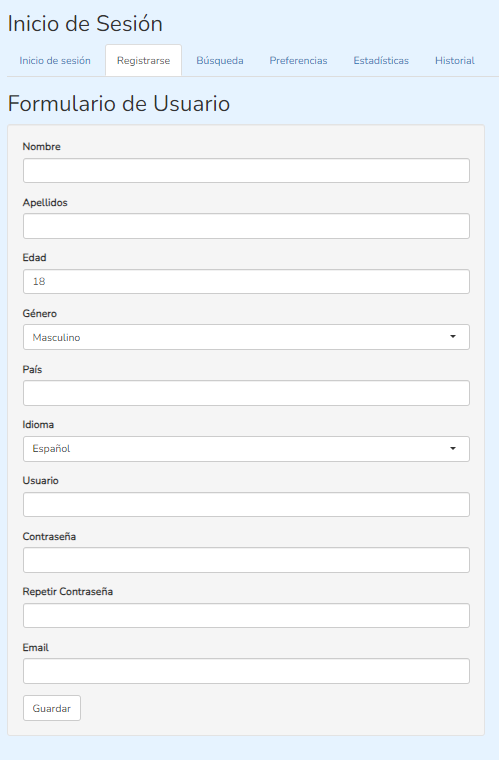
\includegraphics[width=0.5\textwidth]{imagenes/registro.png} 
        \caption{Formulario de registro de usuario}
        \label{fig:ejemplo}
    \end{figure}
 Al iniciar la aplicación por primera vez, el usuario será dirigido automáticamente a la pestaña "Formulario de Usuario" para completar su registro. Este formulario requiere que el usuario proporcione información personal básica, incluyendo su nombre, apellido, edad, género, país e idioma preferido. Además, se le solicita al usuario que elija un nombre de usuario único y una contraseña segura, que deberá ingresar dos veces para asegurar que la haya introducido correctamente, en caso de no hacerlo aparecerá un mensaje de error. También se le pide que ingrese su dirección de correo electrónico para fines de comunicación y recuperación de cuenta. Una vez que todos los campos obligatorios han sido completados, el usuario puede guardar la información haciendo clic en el botón correspondiente.


 \subsection{Inicio de sesión}

 Para acceder a la aplicación, el usuario debe situarse en la pantalla de Inicio de Sesión. En esta pantalla, debe introducir sus credenciales, que consisten en su nombre de usuario y contraseña, en los campos correspondientes. Una vez ingresadas las credenciales, el usuario debe pulsar el botón de \textit{Iniciar Sesión}. Si las credenciales son correctas, aparecerá un mensaje de bienvenida, indicando que el acceso ha sido exitoso.

 \begin{figure}
    \centering
    \includegraphics[width=0.5\textwidth]{imagenes/sesionr.png}
    \caption{Inicio de sesión}
    \label{fig:enter-label}
\end{figure}
 
 \subsection{Gestión de preferencias}
 \begin{figure}
        \centering
        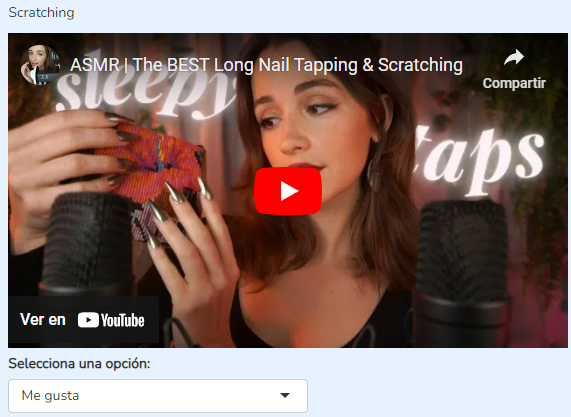
\includegraphics[width=0.5\textwidth]{imagenes/ejemplo_preferencias.png} 
        \caption{Ejemplo de selección de preferencias}
        \label{fig:ejemplo}
    \end{figure}
En la pestaña de Preferencias, el usuario tiene la opción de gestionar qué etiquetas van a aparecer o no en sus búsquedas. Para hacerlo, el usuario debe reproducir todos los vídeos, pudiendo optar por verlos completos o solo una parte de ellos. Tras la visualización de cada vídeo, el usuario debe utilizar el desplegable correspondiente para evaluar su experiencia. Las opciones de evaluación incluyen: si el vídeo le ha gustado y le ha parecido relajante, si no le ha gustado, o si le ha resultado neutral. Una vez completadas todas las evaluaciones, el usuario debe pulsar el botón de "Guardar Preferencias". Al hacerlo, el sistema almacenará sus selecciones, asegurando que sus preferencias sean tenidas en cuenta para futuras interacciones.
 \subsection{Búsqueda}

 En la pestaña de Búsqueda, el usuario debe ingresar el término deseado, preferiblemente precedido por ASMR, el sistema realizará una búsqueda personalizada, teniendo en cuenta las preferencias del usuario. Las etiquetas marcadas como no deseadas por el usuario serán excluidas de los resultados, mientras que aquellas marcadas como favoritas recibirán una mayor prioridad. Los resultados de la búsqueda se presentarán en una tabla que muestra hasta 10 videos relevantes, junto con sus etiquetas asociadas. Para acceder al vídeo seleccionado, el usuario simplemente necesita hacer clic en la URL proporcionada, para ser redireccionado a YouTube.

 \subsection{Vídeos favoritos}
 \begin{figure}
        \centering
        \includegraphics[width=0.5\textwidth]{imagenes/favs.png} 
        \caption{Pestaña de vídeos favoritos}
        \label{fig:ejemplo}
    \end{figure}
 En la pestaña de Vídeos Favoritos, el usuario puede gestionar sus vídeos favoritos introduciendo la URL del vídeo que ha visualizado y desea guardar. Una vez ingresada la URL, el vídeo aparecerá en una tabla junto con el resto de sus vídeos favoritos, mostrando su nombre, URL y etiquetas asociadas. El usuario puede almacenar hasta un máximo de 10 vídeos en esta lista. Además, si desea eliminar un vídeo específico de sus favoritos, puede hacerlo introduciendo la URL correspondiente y pulsando el botón de eliminar. Esto permite al usuario mantener su lista de vídeos favoritos organizada y actualizada según sus preferencias.
 \subsection{Estadísticas de sueño}
  \begin{figure}
        \centering
        \includegraphics[width=0.5\textwidth]{imagenes/registrocompleto.png} 
        \caption{Registro diario de estadísticas de sueño}
        \label{fig:ejemplo}
    \end{figure}
    La pestaña de Estadísticas proporciona al usuario un análisis detallado de su calidad de sueño. Para registrar su información, se le solicita al usuario que ingrese la fecha correspondiente, el número de horas dormidas durante la noche anterior, así como el número de despertares experimentados. Además, se le solicita describir la sensación con la que se despierta, seleccionando entre las opciones de \textit{cansado}, \textit{descansado}, o \textit{normal}. También se registra la hora de apagado y encendido de luces, lo que proporciona un contexto importante para analizar los hábitos de sueño. A continuación tiene la opción para marcar si ha experimentado un despertar precoz, es decir, si se ha despertado antes de que suene el despertador. Esto ayuda a identificar patrones de sueño interrumpidos. Además, se solicita al usuario que registre la latencia de sueño en minutos, que es el tiempo que transcurre desde que se apagan las luces hasta que se concilia el sueño. Esta métrica permite evaluar la eficiencia para dormir. Las estadísticas que se obtienen se pueden utilizar en la consulta clínica para evaluar su proceso de tratamiento.
 \section{Demostración práctica de uso. Administrador}
 \begin{figure}
    \centering
    \includegraphics[width=0.75\textwidth]{imagenes/admin.png}
    \caption{Vista del administrador}
    \label{fig:enter-label}
\end{figure}
El rol de administrador otorga al usuario privilegios adicionales para gestionar la aplicación de manera integral. Para acceder a las funciones de administración, el administrador debe autenticarse utilizando sus credenciales correspondientes. Una vez dentro de la pestaña de Administrador, se le presenta una tabla que enumera los usuarios registrados, incluyendo su nombre, apellido y dirección de correo electrónico asociada. Puede crear un nuevo usuario proporcionando todos los datos necesarios para su registro tras pulsar el botón crear, para el resto de opciones tiene la opción de buscar un usuario específico ingresando su dirección de correo electrónico, lo que le permite modificar los detalles existentes, consultar la información asociada o eliminar la cuenta. Esta funcionalidad brinda al administrador un control completo sobre la gestión de usuarios.

\apendice{Manual del programador}
\section{Estructura de directorios}
Este apartado incluye la información relativa a la organización del repositorio del proyecto, disponible en \url{https://github.com/rocioalonsolh/tfg-asmr} donde los directorios se estructuran de la siguiente manera:
\begin{itemize}
    \item /: Directorio raíz, en él se encuentran el archivo README y las carpetas que engloban el proyecto (documentación, aplicación y base de datos)
    \item /app: La carpeta correspondiente a la aplicación, en ella se encuentra el código R de la misma y el css del frontend.
    \item /app/shiny.R: Código R de la aplicación Shiny final.
    \item /app/estilo.css: Código relativo al estilo de la aplicación.
    \item /bbdd: Carpeta empleada para guardar las bases de datos, en esta versión preliminar solamente incluye una.
    \item /bbdd/usuarios: Base de datos con toda la información de los usuarios, sus preferencias, estadísticas y vídeos favoritos.
    \item /docs: Módulo que contiene la documentación del proyecto.
    \item /docs/tex: Carpeta con los documentos de memoria, anexos y bibliografía en formato \LaTeX.
    \item /docs/pdf: Carpeta con el documento en pdf de la memoria y del anexo.
    \item /docs/img: Carpeta con las imágenes empleadas en la documentación del proyecto.
\end{itemize}
Las carpetas descritas son las necesarias para ejecutar el proyecto, además se encuentran en el repositorio otros documentos que fueron parte del proceso y que sin ser necesarios, podrían resultar de ayuda.
\section{Entorno de desarrollo}
En este apartado se detallan los elementos utilizados para el desarrollo del programa, que deberían tenerse en cuenta a la hora de trabajar sobre él, para mantener la coherencia.
\begin{itemize}
    \item R 4.4.0
    \item RStudio
    \item Bibliotecas R
    \item Visual Studio
\end{itemize}
\subsection{R 4.4.0} Versión del lenguaje R \cite{R}
\subsection{RStudio} Entorno de desarrollo integrado (IDE) para el lenguaje de programación R, especializado en computación estadística y gráficos. Utilizado para desarrollar la aplicación Shiny. 
 \begin{figure}
    \centering
    \includegraphics[width=1\textwidth]{imagenes/vgrstudio.png}
    \caption{Visión General IDE RStudio}
    \label{fig:enter-label}
\end{figure}
\subsection{Bibliotecas R}
Las bibliotecas R que han sido utilizadas y que por tanto han de ser cargadas de manera previa para poder trabajar en el proyecto son: 
\begin{itemize}
    \item \textit{shiny} Para crear la aplicación
    \item \textit{shinyWidgets} Para disponer de más widgets
    \item \textit{tuber} Para la conexión con YouTube Data API
    \item \textit{dplyr} Para tratamiento de datos
    \item \textit{stringr} Para tratamiento de cadenas
    \item \textit{magrittr} Para introducir el operador de tuberías \%>\%
    \item \textit{DBI} Para interactuar con las bases de datos
    \item \textit{RSQLite} Para trabajar con bases de datos SQLite
    \item \textit{ggplot2} Para creación de gráficos
    \item \textit{purrr} Para programación funcional
\end{itemize}
\subsection{Visual Studio} Visual Studio se ha utilizado para crear y manipular el archivo de estilo, aunque no es necesario, podría modificarse desde cualquier otro IDE o editor de texto.

\section{Compilación, instalación y ejecución del proyecto}
Para compilar, instalar y ejecutar el proyecto es necesario seguir los siguientes pasos:
\subsection{Paso 1. Descarga de los archivos}
Se accederá al repositorio (\url{https://github.com/rocioalonsolh/tfg-asmr}) para descargar todo el contenido de la carpeta app, el contenido de bbdd, y adicionalmente se puede descargar todo el contenido restante, aunque no es necesario para la utilización de la app.
\subsection{Paso 2. Instalación de R y RStudio}
En caso de no tener instalados el lenguaje y el IDE de manera previa, será necesario descargarlos e instalarlos, se encuentran disponibles en:
\begin{itemize}
    \item R 4.4.0 https://cran.rediris.es/
    \item RStudio https://posit.co/download/rstudio-desktop/
\end{itemize}
\subsection{Paso 3. Obtención de credenciales YouTube Data API} Para El correcto funcionamiento de la aplicación es necesario obtener credenciales mediante Google Console.
\begin{itemize}
  \item Crear un proyecto en la Consola de Desarrolladores de Google. \url{https://console.cloud.google.com/}
  \item Habilitar la API de YouTube Data.
   \begin{figure}
    \centering
    \includegraphics[width=1\textwidth]{imagenes/ytdahabilitada.png}
    \caption{Pantalla de habilitación Youtube Data API}
    \label{fig:enter-label}
\end{figure}
  \item Crea credenciales de autenticación, OAuth 2.0 client ID, para aplicación web.
  \begin{figure}
    \centering
    \includegraphics[width=1\textwidth]{imagenes/creacioncredenciales.png}
    \caption{Creación de credenciales desde Google Console}
    \label{fig:enter-label}
\end{figure}
  \item Configurar las restricciones de la API y las claves.
  \item Descargar o copiar la clave de API o el archivo JSON de credenciales (han de ser almacenados de manera segura).
  \item En caso de haber copiado el ID de cliente y el secreto de cliente, sustituirlos al comienzo del código, en caso de optar por el JSON, incluirlo en el mismo.
  \begin{figure}
    \centering
    \includegraphics[width=0.75\textwidth]{imagenes/codigoauth.png}
    \caption{Establecimiento de credenciales desde R}
    \label{fig:enter-label}
\end{figure}
\end{itemize}
\subsection{Paso 4. Instalación de DB Browser for SQLite} Una vez creada la base de datos es posible trabajar con ella directamente desde RStudio, en cualquier caso, por facilidad y coherencia con el proyecto, se recomienda utilizar para trabajar con la base de datos la misma herramienta que durante el desarrollo, disponible en https://sqlitebrowser.org/.

\subsection{Paso 5. Cambiar la ruta de la base de datos en el código}
Para poder trabajar correctamente con la app, será necesario modificar la parte del código en la que se especifica la manera de llevar a cabo la conexión con la base de datos, y redirigir la ruta al directorio en el que se haya guardado el archivo usuarios.db.

\subsection{Paso 6. Ejecución}
Una vez llavados a cabo todos los pasos anteriores puede procederse a ejecutar la app, por defecto en un puerto local, con posibles modificaciones en versiones futuras.

\section{Pruebas del sistema}
\subsection{Inicio de sesión}
En el inicio de sesión será necesario realizar dos pruebas, una con credenciales correctas y otra con credenciales incorrectas, para comprobar la respuesta de la app. Las credenciales que se han utilizado durante la fase de pruebas han sido 
Usuario: roci@email.com
Contraseña: roci
En caso de modificar la base de datos, comprobar que se están utilizando unas credenciales correctas.
 \begin{figure}
    \centering
    \includegraphics[width=1\textwidth]{imagenes/isbueno.jpg}
    \caption{Ejemplo de inicio correcto de sesión}
    \label{fig:enter-label}
\end{figure}
 \begin{figure}
    \centering
    \includegraphics[width=1\textwidth]{imagenes/ismalo.jpg}
    \caption{Ejemplo de inicio de sesión fallido}
    \label{fig:enter-label}
\end{figure}
Una vez iniciada la sesión es necesario comprobar en el resto de pestañas si los registros que aparecen concuerdan con los del usuario seleccionado.
\subsection{Registro de usuario}
Las pruebas relativas a esta sección requieren 3, las posibilidades de entrada de datos son limitadas para los usuarios, por lo que solo pueden presentarse 2 posibles errores.
\begin{enumerate}
    \item Introducir datos correctos, comprobar que se actualiza la tabla.
    \item Introducir la repetición de la contraseña de manera incorrecta, esperar el mensaje de error.
     \begin{figure}
    \centering
    \includegraphics[width=1\textwidth]{imagenes/registromalo.jpg}
    \caption{Mensaje de error por repetición incorrecta de contraseña}
    \label{fig:enter-label}
\end{figure}
    \item Introducir un correo ya presente en la base de datos, el registro no se llevará a cabo.  
\end{enumerate}
\subsection{Preferencias}
Marcar los botones de la pestaña de preferencias y pulsar el botón de guardarcomprobar en la tabla que los datos se guardan correctamente.

\subsection{Búsqueda}
Comprobar que los datos de etiquetas marcadas como \textit{Me gusta} y \textit{No me gusta} corresponden con el usuario seleccionado. Introducir un término de búsqueda, comprobar que la salida son 10 registros con etiquetas y que los hipervínculos funcionan.

\subsection{Favoritos}
Añadir un vídeo a favoritos. Eliminar un vídeo de la tabla. Comprobar que la base de datos tras estas dos acciones se ha actualizado correctamente.

\subsection{Administrador}
Acceder con credenciales de administrador, visualizar la tabla con los datos, llevar a cabo las 4 operaciones posibles, comprobar que los cambios se guardan.
\begin{figure}
    \centering
    \includegraphics[width=1\textwidth]{imagenes/admin.png}
    \caption{Opciones administrador}
    \label{fig:enter-label}
\end{figure}
\section{Instrucciones para la modificación o mejora del proyecto}
En esta sección se detallaran los puntos a tener en cuenta en caso de realizar mejoras o modificaciones a la aplicación.

El punto más relevante es mantener las modificaciones de código claramente documentadas de manera exhaustiva, con los comentarios pertinentes o informes adicionales, para que sea comprensible por otros programadores. Los comentarios deben ser claros y concisos.

En caso de añadir nuevas funcionalidades, ha de documentarse el procedimiento esperado para llevar a cabo las pruebas al probar la aplicación desde nuevos equipos.

Con la aplicación funcionando de manera real, los datos recogidos serán de carácter sensible, por lo que se implementarán medidas de seguridad para tratarlos.

Las mejoras o modificaciones realizadas serán subidas al repositorio original, con el propósito de mantener la aplicación accesible.

\apendice{Descripción de adquisición y tratamiento de los datos}
\section{Descripción formal de los datos}
\subsection{Datos usuarios}
Los datos relativos a \textbf{usuarios}, que serían obtenidos en la fase de explotación, durante el desarrollo de este proyecto han sido parte de elaboración propia y algunos se han obtenido solicitándolos a ChatGPT, como se ha mencionado en la memoria del proyecto. Los datos de los usuarios incluyen:
\begin{enumerate}
    \item Nombre
    \item Apellidos
    \item Edad
    \item País
    \item Idioma
    \item Género
    \item Correo electrónico
    \item Contraseña
    \item Usuario
\end{enumerate}

Los datos de \textbf{preferencias} han sido completamente de elaboración propia, obtenidos completando el formulario para poder comprobar como se guardaban con cada registro, estos datos incluyen valores positivos, negativos o neutros que valoran los 10 estímulos seleccionados.

Dado que estos datos han sido creados específicamente para el proyecto, no ha sido necesario realizar un tratamiento sobre ellos para limpiarlos o transformarlos, las contraseñas se guardaron como texto, se podría considerar en futuras mejoras el encriptarlas.

En cuanto a tamaño, se crearon 20 registros iniciales de usuarios falsos, sobre los que después se añadieron y quitaron algunos durante las fases de pruebas de la aplicación. En caso de que la aplicación se pusiera en funcionamiento, habría que replantear ciertos aspectos del almacenamiento de los datos. dado que durante el desarrollo del proyecto se trabajaba con un número tan limitado de registros que el espacio que ocupaban los datos no presentaba un problema.

Por último, los datos relativos a los vídeos, han sido obtenidos directamente de Youtube a través de Youtube Data API, realizando la conexión desde R con el paquete \textit{tuber}. Los datos se han recolectado realizando las búsquedas, y solamente se han guardado en la base de datos de vídeos favoritos algunos escogidos manualmente por ser considerados ejemplos de interés. Se obtuvieron los metadatos del vídeo y los no relevantes (como algunos relacionados con las dechas de publicación o interacciones fueron descartados por falta de interés), los que se guardaron fueron:
\begin{enumerate}
    \item Nombre del vídeo
    \item URL
    \item Etiquetas
    \item Nombre del canal
    \item Identificador
\end{enumerate}

La limpieza de datos se llevó a cabo directamente desde la búsqueda, eliminando aquellos vídeos que no contenían etiquetas, por falta de detalles específicos para la aplicación.

Se obtuvieron los datos dentro de los términos de servicio y las políticas de privacidad de YouTube durante la obtención de los metadatos de los vídeos. Se ha garantizado el uso ético de los datos recopilados, asegurando la protección de la privacidad de los usuarios y el respeto a los derechos de autor.

\section{Descripción clínica de los datos}
Los datos de \textbf{estadísticas} son los únicos que guardan relevancia clínica, debido a que son los que serán necesarios para hacer el seguimiento del tratamiento y evolución del paciente, los usados han sido completamente de elaboración propia, obtenidos completando el formulario para poder comprobar como evolucionaban las gráficas, estos datos incluyen:
\begin{enumerate}
    \item Horas de sueño
    \item Sensación al despertar
    \item Número de despertares
    \item Hora de apagado de luces
    \item Hora de encendido de luces
    \item Despertar precoz
    \item Latencia de sueño
\end{enumerate}

Es necesario resaltar que los datos obtenidos de usuarios reales en fases futuras serán considerados datos protegidos por ser de carácter médico, por tanto legislativamente están regulados por la Ley Orgánica 3/2018, de 5 de diciembre, de Protección de Datos Personales y garantía de los derechos digitales (LOPDGDD), que incorpora disposiciones del Reglamento General de Protección de Datos (GDPR) de la Unión Europea. \cite{boe-2018} Debido a esto, los usuarios deberán dar consentimiento expreso para el tratamiento de sus datos.
\apendice{Especificación de diseño}
\section{Estructura de la aplicación}
\begin{enumerate}
    \item Inicio de Sesión:
    \begin{itemize}
        \item Permite a los usuarios guardar sus datos y preferencias.
    \end{itemize}
    
    \item Registro:
    \begin{itemize}
        \item Preguntas sobre los datos personales del usuario.
        \item Almacena las respuestas para crear una cuenta.
    \end{itemize}
    
    \item Preferencias:
    \begin{itemize}
        \item Permite a los usuarios introducir o ajustar sus preferencias en cualquier momento.
    \end{itemize}
    
    \item Búsqueda Específica:
    \begin{itemize}
        \item Permite a los usuarios buscar videos de ASMR filtrando por etiquetas específicas.
        \item Integra la YouTube Data API para realizar búsquedas.
    \end{itemize}
    
    \item Favoritos:
    \begin{itemize}
        \item Lista de videos marcados como favoritos por el usuario.
        \item Acceso sencillo a los vídeos marcados.
    \end{itemize}
\end{enumerate}
\section{Diagramas de procesos}
En esta seccion se presentan los diagramas de los principales procesos que se dan en la aplicación, descritos mediante BPMN.
\begin{figure}
    \centering
    \includegraphics[width=0.5\textwidth]{imagenes/cu1.png}
    \caption{Diagrama de proceso. Registro de usuarios}
    \label{fig:enter-label}
\end{figure}
\begin{figure}
    \centering
    \includegraphics[width=1\textwidth]{imagenes/cu2.png}
    \caption{Diagrama de proceso. Primer uso de la aplicación}
    \label{fig:enter-label}
\end{figure}
\begin{figure}
    \centering
    \includegraphics[width=1\textwidth]{imagenes/cu3.png}
    \caption{Diagrama de proceso. Inicio de sesión normal}
    \label{fig:enter-label}
\end{figure}
\begin{figure}
    \centering
    \includegraphics[width=1\textwidth]{imagenes/cu4.png}
    \caption{Diagrama de proceso. Búsqueda}
    \label{fig:enter-label}
\end{figure}

\section{Diagrama de las bases de datos}
En la figura E.5 se encuentra una descripción visual de la base de datos.
 \begin{figure}
    \centering
    \includegraphics[width=1\textwidth]{imagenes/esquemabbdd.png}
    \caption{Diagrama de la base de datos. Realizado con Luna Modeler}
    \label{fig:enter-label}
\end{figure}

\section{Descripción de la base de datos}
La base de datos se compone de 4 tablas distintas, descritas a continuación:
\subsection*{Tabla: Usuarios}
\begin{itemize}
  \item \textbf{email (Clave Primaria):} Texto. Dirección de correo electrónico única para identificar a cada usuario.
  \item \textbf{id:} Numérico. Identificador único para cada usuario, asignado automáticamente.
  \item \textbf{nombre:} Texto. Nombre del usuario.
  \item \textbf{apellido:} Texto. Apellido del usuario.
  \item \textbf{edad:} Numérico. Edad del usuario.
  \item \textbf{género:} Texto. Género del usuario.
  \item \textbf{país:} Texto. País de residencia del usuario.
  \item \textbf{idioma:} Texto. Idioma preferido del usuario.
  \item \textbf{usuario:} Texto. Nombre de usuario único para iniciar sesión.
  \item \textbf{contraseña:} Texto. Contraseña para iniciar sesión.
\end{itemize}

\subsection*{Tabla: Estadísticas}
\begin{itemize}
  \item \textbf{id (Clave Primaria):} Numérico. Identificador único para cada registro de estadísticas, asignado automáticamente.
  \item \textbf{email:} Texto. Dirección de correo electrónico del usuario al que pertenecen las estadísticas.
  \item \textbf{fecha:} Texto. Fecha de registro de las estadísticas.
  \item \textbf{horas\_sueño:} Numérico. Cantidad de horas de sueño del usuario.
  \item \textbf{despertares:} Numérico. Número de veces que el usuario se despierta durante el sueño.
  \item \textbf{sensación:} Texto. Descripción de la sensación del usuario al despertar.
  \item \textbf{apagado\_de\_luces:} Texto. Estado de las luces al dormir (encendidas/apagadas).
  \item \textbf{encendido\_de\_luces:} Texto. Estado de las luces al despertar (encendidas/apagadas).
  \item \textbf{despertar\_precoz:} Texto. Descripción de si el usuario se despertó antes de lo esperado.
  \item \textbf{latencia\_de\_sueño:} Numérico. Tiempo que tarda el usuario en conciliar el sueño.
\end{itemize}

\subsection*{Tabla: Videosfav}
\begin{itemize}
  \item \textbf{URL (Clave Primaria):} Texto. Dirección única de URL del video favorito.
  \item \textbf{usuario:} Texto. Nombre de usuario del usuario que marcó el video como favorito.
  \item \textbf{nombre:} Texto. Nombre del video favorito.
  \item \textbf{etiquetas:} Texto. Etiquetas o categorías asociadas al video favorito.
\end{itemize}

\subsection*{Tabla: Preferencias}
\begin{itemize}
  \item \textbf{email (Clave Primaria):} Texto. Dirección de correo electrónico única para identificar las preferencias de cada usuario.
  \item \textbf{susurros:} Texto. Preferencia del usuario por los sonidos de susurros.
  \item \textbf{scratching:} Texto. Preferencia del usuario por los sonidos de rasguños.
  \item \textbf{juego\_rol:} Texto. Preferencia del usuario por los vídeos relacionados con juegos de rol.
  \item \textbf{sonidos\_boca:} Texto. Preferencia del usuario por los sonidos bucales.
  \item \textbf{toques:} Texto. Preferencia del usuario por los sonidos de toques.
  \item \textbf{susurros\_inaudibles:} Texto. Preferencia del usuario por los susurros inaudibles.
  \item \textbf{movimientos\_lentos:} Texto. Preferencia del usuario por los vídeos de movimientos lentos.
  \item \textbf{masajes:} Texto. Preferencia del usuario por los vídeos de masajes.
  \item \textbf{visual:} Texto. Preferencia del usuario por la estimulación visual.
\end{itemize}

\apendice{Especificación de requisitos}
\section{Diagramas de casos de Uso}
Se describen visualmente a continuación los casos de uso principales de la aplicación.
\begin{figure}
    \centering
    \includegraphics[width=0.75\textwidth]{imagenes/casos de uso.png}
    \caption{Diagrama casos de uso}
    \label{fig:enter-label}
\end{figure}

\begin{table}[h!]
\centering
\begin{tabular}{ll}
\toprule
\textbf{CU 1} & \textbf{Registro} \\
\midrule
\textbf{Versión} & 1.0 \\
\textbf{Autor} & Rocío Alonso \\
\textbf{Descripción} & Registro de un usuario nuevo \\
\textbf{Precondición} & Iniciar la aplicación \\
\textbf{Acciones} & 
\begin{tabular}[t]{@{}l@{}}
    1. Introducir los datos del usuario \\
    2. Pulsar el botón de registro
\end{tabular} \\
\textbf{Postcondición} & Nuevo usuario registrado \\
\textbf{Excepciones} & 
\begin{tabular}[t]{@{}l@{}}
    \textbullet\ Las contraseñas no coinciden \\
    \textbullet\ El email del usuario se repite
\end{tabular} \\
\textbf{Importancia} & Alta \\
\bottomrule
\end{tabular}
\caption{CU 1 - Registro de un nuevo usuario}
\label{tabla-cu1}
\end{table}

\begin{table}[h!]
\centering
\begin{tabular}{ll}
\toprule
\textbf{CU 2} & \textbf{Inicio de sesión} \\
\midrule
\textbf{Versión} & 1.0 \\
\textbf{Autor} & Rocío Alonso \\
\textbf{Descripción} & Introducción de credenciales para ingresar en la aplicación\\
\textbf{Precondición} & El usuario debe estar registrado de manera previa\\
\textbf{Acciones} & 
\begin{tabular}[t]{@{}l@{}}
    1. Introducir usuario y contraseña\\
    2. Pulsar el botón de ingreso
\end{tabular} \\
\textbf{Postcondición} & Acceso a la aplicación concedido \\
\textbf{Excepciones} & 
\begin{tabular}[t]{@{}l@{}}
    \textbullet\ Las credenciales no son válidas \\
\end{tabular} \\
\textbf{Importancia} & Alta \\
\bottomrule
\end{tabular}
\caption{CU 2 - Inicio de sesión}
\label{tabla-cu1}
\end{table}

\begin{table}[h!]
\centering
\begin{tabular}{ll}
\toprule
\textbf{CU 3} & \textbf{Preferencias} \\
\midrule
\textbf{Versión} & 1.0 \\
\textbf{Autor} & Rocío Alonso \\
\textbf{Descripción} & Visualización de los vídeos seleccionados para su evaluación\\
\textbf{Precondición} & El usuario debe haber accedido correctamente a la aplicación\\
\textbf{Acciones} & 
\begin{tabular}[t]{@{}l@{}}
    1. Visualizar los vídeos seleccionados\\
    2. Evaluar los vídeos vistos
\end{tabular} \\
\textbf{Postcondición} & Nuevo registro de preferencias \\
\textbf{Excepciones} & 
\begin{tabular}[t]{@{}l@{}}
\end{tabular} \\
\textbf{Importancia} & Media \\
\bottomrule
\end{tabular}
\caption{CU 3 - Registro de preferencias}
\label{tabla-cu3}
\end{table}

\begin{table}[h!]
\centering
\begin{tabular}{ll}
\toprule
\textbf{CU 4} & \textbf{Búsqueda} \\
\midrule
\textbf{Versión} & 1.0 \\
\textbf{Autor} & Rocío Alonso \\
\textbf{Descripción} & Ejecución de la búsqueda\\
\textbf{Precondición} & El usuario debe haber accedido correctamente a la aplicacións\\
\textbf{Acciones} & 
\begin{tabular}[t]{@{}l@{}}
    1. Introducir el término de búsqueda\\
    2. Ejecutar la búsqueda\\
    3. Seleccionar vídeo
\end{tabular} \\
\textbf{Postcondición} & Usuario derivado a YouTube \\
\textbf{Excepciones} & 
\begin{tabular}[t]{@{}l@{}}
    \textbullet\ La búsqueda está saturada \\
\end{tabular} \\
\textbf{Importancia} & Alta \\
\bottomrule
\end{tabular}
\caption{CU 4 - Búsqueda}
\label{tabla-cu4}
\end{table}

\begin{table}[h!]
\centering
\begin{tabular}{ll}
\toprule
\textbf{CU 5.1} & \textbf{Consultar estadísticas} \\
\midrule
\textbf{Versión} & 1.0 \\
\textbf{Autor} & Rocío Alonso \\
\textbf{Descripción} & Visualización de las gráficas de sueño\\
\textbf{Precondición} & El usuario debe haber accedido correctamente a la aplicación\\
\textbf{Acciones} & 
\begin{tabular}[t]{@{}l@{}}
    1. Acceder a la pestaña de estadísticas\\
    2. Pulsar el botón de visualización de estadícas
\end{tabular} \\
\textbf{Postcondición} & Gráficas mostradas \\
\textbf{Excepciones} & 
\begin{tabular}[t]{@{}l@{}}
    \textbullet\ No existen registros previos \\
\end{tabular} \\
\textbf{Importancia} & Media \\
\bottomrule
\end{tabular}
\caption{CU 5.1 - Consultar Estadísticas}
\label{tabla-cu51}
\end{table}

\begin{table}[h!]
\centering
\begin{tabular}{ll}
\toprule
\textbf{CU 5.2} & \textbf{Introducir datos estadísticas} \\
\midrule
\textbf{Versión} & 1.0 \\
\textbf{Autor} & Rocío Alonso \\
\textbf{Descripción} & El usuario introduce los datos de la noche anterior
\\
\textbf{Precondición} & El usuario debe haber accedido correctamente a la aplicación\\
\textbf{Acciones} & 
\begin{tabular}[t]{@{}l@{}}
    1. Introducir datos de sueño\\
    2. Pulsar el botón guardado
\end{tabular} \\
\textbf{Postcondición} & Registro de sueño guardado \\
\textbf{Excepciones} & 
\begin{tabular}[t]{@{}l@{}}
\end{tabular} \\
\textbf{Importancia} & Media \\
\bottomrule
\end{tabular}
\caption{CU 5.2 - Introducir datos estadísticas}
\label{tabla-cu51}
\end{table}

\begin{table}[h!]
\centering
\begin{tabular}{ll}
\toprule
\textbf{CU 6.1} & \textbf{Consultar pestaña Favoritos} \\
\midrule
\textbf{Versión} & 1.0 \\
\textbf{Autor} & Rocío Alonso \\
\textbf{Descripción} & El usuario consulta sus videos guardados como favoritos
\\
\textbf{Precondición} & El usuario debe haber accedido correctamente a la aplicación\\
\textbf{Acciones} & 
\begin{tabular}[t]{@{}l@{}}
    1. Acceder a la pestaña de favoritos\\
    2. Seleccionar un vídeo de los guardados
\end{tabular} \\
\textbf{Postcondición} & Usuario derivado a YouTube \\
\textbf{Excepciones} & 
\begin{tabular}[t]{@{}l@{}}
    \textbullet\ No hay vídeos guardados en favoritos \\
\end{tabular} \\
\textbf{Importancia} & Baja \\
\bottomrule
\end{tabular}
\caption{CU 6.1 - Consultar pestaña Favoritos}
\label{tabla-cu61}
\end{table}

\begin{table}[h!]
\centering
\begin{tabular}{ll}
\toprule
\textbf{CU 6.2} & \textbf{Introducir vídeo nuevo en Favoritos} \\
\midrule
\textbf{Versión} & 1.0 \\
\textbf{Autor} & Rocío Alonso \\
\textbf{Descripción} & El usuario introduce un nuevo vídeo de en sus favoritos
\\
\textbf{Precondición} & El usuario debe haber accedido correctamente a la aplicación\\
\textbf{Acciones} & 
\begin{tabular}[t]{@{}l@{}}
    1. Acceder a la pestaña de favoritos\\
    2. Introducir la URL del video para añadir
\end{tabular} \\
\textbf{Postcondición} & Tabla de favoritos actualizada \\
\textbf{Excepciones} & 
\begin{tabular}[t]{@{}l@{}}
    \textbullet\ La URL no es válida \\
\end{tabular} \\
\textbf{Importancia} & Baja \\
\bottomrule
\end{tabular}
\caption{CU 6.2 - Introducir vídeo nuevo en Favoritos}
\label{tabla-cu62}
\end{table}

\begin{table}[h!]
\centering
\begin{tabular}{ll}
\toprule
\textbf{CU 6.3} & \textbf{Eliminar vídeo de Favoritos} \\
\midrule
\textbf{Versión} & 1.0 \\
\textbf{Autor} & Rocío Alonso \\
\textbf{Descripción} & El usuario elimina un vídeo de en sus favoritos
\\
\textbf{Precondición} & El usuario debe haber accedido correctamente a la aplicación\\
\textbf{Acciones} & 
\begin{tabular}[t]{@{}l@{}}
    1. Acceder a la pestaña de favoritos\\
    2. Introducir la URL del video para eliminarlo
\end{tabular} \\
\textbf{Postcondición} & Tabla de favoritos actualizada \\
\textbf{Excepciones} & 
\begin{tabular}[t]{@{}l@{}}
    \textbullet\ La URL no es válida \\
    \textbullet\ No hay registros en la tabla \\
\end{tabular} \\
\textbf{Importancia} & Baja \\
\bottomrule
\end{tabular}
\caption{CU 6.3 - Eliminar un vídeo de Favoritos}
\label{tabla-cu63}
\end{table}



\apendice{Anexo sobre sostenibilización curricular}
La sostenibilización curricular de este Trabajo de Fin de Grado (TFG) está basada en el principio de accesibilidad universal y diseño para todas las personas, conforme a lo establecido en la disposición final segunda del Texto Refundido de la Ley General de las personas con discapacidad y de su inclusión social, aprobado por Real Decreto legislativo 1/2013 del 29 de noviembre. \cite{boe-2013}

\section{Relación con los Principios de Accesibilidad Universal}
La aplicación desarrollada como parte de este TFG, ASMR Sleep, destinada inicialmente a personas con insomnio de conciliación, ha sido concebida con un enfoque inclusivo y accesible para todas las personas. A través de un diseño intuitivo y funcional, se busca garantizar que cualquier usuario, independientemente de sus capacidades físicas o cognitivas, pueda utilizarla de manera efectiva.

\subsection{Adaptación para Personas con Discapacidad}
La accesibilidad de la aplicación se ha abordado desde la perspectiva del diseño centrado en el usuario, la interfaz se ha guiado por principios de diseño centrado en el usuario, con énfasis en la claridad, la simplicidad y la consistencia, lo que facilita la navegación para personas con discapacidad cognitiva o dificultades de aprendiz para asegurar su utilidad para un amplio espectro de usuarios, como aquellos con discapacidades cognitivas o dificultades de aprendizaje.

\subsection{Contribución a la Inclusión Social}
Además de su enfoque en la accesibilidad, la aplicación también promueve la inclusión social al proporcionar una herramienta de apoyo gratuita para personas con insomnio de conciliación. Al facilitar el acceso a contenido de ASMR, la aplicación busca mejorar la calidad del sueño y el bienestar general de sus usuarios, independientemente de sus circunstancias individuales.

\subsection{Ampliación de Beneficios a toda la Población}
Si bien la aplicación se desarrolló inicialmente con un público específico en mente, su diseño y funcionalidades son fácilmente generalizables a toda la población. Esto se alinea con el principio de diseño para todas las personas, asegurando que los beneficios de la aplicación no estén limitados a un grupo particular, sino que estén disponibles para cualquier individuo que busque mejorar su calidad de vida mediante técnicas de relajación y bienestar.

En resumen, la sostenibilización curricular de este TFG se refleja en el compromiso con la accesibilidad universal y la inclusión social, garantizando que la aplicación desarrollada sea una herramienta efectiva y accesible para todos los usuarios, en consonancia con los principios establecidos en la legislación vigente sobre discapacidad y inclusión social.



 
\include{./tex/A_planificacion}
\include{./tex/B_manual_usuario}
\include{./tex/C_manual_programador}
\include{./tex/D_datos}
\include{./tex/E_diseno}
\include{./tex/F_requisitos}
\include{./tex/G_experimental}
\include{./tex/H_ODS}



\bibliographystyle{apalike}
\bibliography{bibliografiaAnexos}

\end{document}